% mnras_template.tex 
%
% LaTeX template for creating an MNRAS paper
%
% v3.0 released 14 May 2015
% (version numbers match those of mnras.cls)
%
% Copyright (C) Royal Astronomical Society 2015
% Authors:
% Keith T. Smith (Royal Astronomical Society)

% Change log
%
% v3.0 May 2015
%    Renamed to match the new package name
%    Version number matches mnras.cls
%    A few minor tweaks to wording
% v1.0 September 2013
%    Beta testing only - never publicly released
%    First version: a simple (ish) template for creating an MNRAS paper

%%%%%%%%%%%%%%%%%%%%%%%%%%%%%%%%%%%%%%%%%%%%%%%%%%
% Basic setup. Most papers should leave these options alone.
\documentclass[fleqn,usenatbib]{mnras}

% MNRAS is set in Times font. If you don't have this installed (most LaTeX
% installations will be fine) or prefer the old Computer Modern fonts, comment
% out the following line
\usepackage{newtxtext,newtxmath}
% Depending on your LaTeX fonts installation, you might get better results with one of these:
%\usepackage{mathptmx}
%\usepackage{txfonts}

% Use vector fonts, so it zooms properly in on-screen viewing software
% Don't change these lines unless you know what you are doing
\usepackage[T1]{fontenc}
\usepackage{subfig} %for figure subplot
\usepackage{graphicx}
\usepackage[flushleft]{threeparttable}
\usepackage{xspace}



%%%%%%%%%%%%%%%%%%%%%%%%%%%%%%%%%%%%%%%%%%%%%%%%%%%%%%%%%%%%%%%%%%%
% my commands
\newcommand{\lcdm}{$\Lambda$CDM}
\newcommand{\hst}{{\it HST}}
\newcommand{\efr}{$R_{\mathrm{eff}}$}
\newcommand{\galfit}{{\sc Galfit}}
\newcommand{\mbh}{$\mathcal M_{\rm BH}$}
\newcommand{\lhost}{$L_{\rm host}$}
\newcommand{\mr}{$Mag_{\rm ~R}$}
\newcommand{\halpha}{H$_{\alpha}$}
\newcommand{\Hb}{H$_{\beta}$}
\newcommand{\sersic}{S\'ersic}
\newcommand{\lenstronomy}{{\sc Lenstronomy}}
\newcommand{\reff}{{$R_{\mathrm{eff}}$}}
\newcommand{\kmsMpc}{km~s$^{\rm -1}$~Mpc$^{\rm -1}$}
\newcommand{\kms}{\ifmmode{\,\rm{km}\, \rm{s}^{-1}}\else{$\,$km$\,$s$^{-1}$}\fi}
\newcommand{\sigstar}{{$\sigma_*$}}
\newcommand{\mstar}{{$M_*$}}
\newcommand{\Mgii}{Mg$_{\rm II}$}
\newcommand{\Civ}{C$_{\rm IV}$}
%\newcommand{\farcs}{\mbox{\ensuremath{.\!\!^{\prime\prime}}}}% fractional arcsecond symbol: 0.''0
\newcommand{\sam}{\texttt{SAM}}
\newcommand{\mbii}{\texttt{MBII}}
%%%%%%%%%%%%%%%%%%%%%%%%%%%%%%%%%%%%%%%%%%%%%%%%%%%%%%%%%%%%%%%%%%%
\newcommand{\ding}[1]{\textcolor{red}{[{\bf Xuheng}: #1]}}
\newcommand{\todo}[1]{\textcolor{red}{[{\bf Todo}: #1]}}  
\newcommand{\red}[1]{{ \textcolor{red}{#1}}}
\newcommand{\blue}[1]{{ \textcolor{blue}{#1}}}
\newcommand{\pink}[1]{{ \textcolor{magenta}{#1}}}

% Allow "Thomas van Noord" and "Simon de Laguarde" and alike to be sorted by "N" and "L" etc. in the bibliography.
% Write the name in the bibliography as "\VAN{Noord}{Van}{van} Noord, Thomas"
\DeclareRobustCommand{\VAN}[3]{#2}
\let\VANthebibliography\thebibliography
\def\thebibliography{\DeclareRobustCommand{\VAN}[3]{##3}\VANthebibliography}


%%%%% AUTHORS - PLACE YOUR OWN PACKAGES HERE %%%%%

% Only include extra packages if you really need them. Common packages are:
\usepackage{graphicx}	% Including figure files
\usepackage{amsmath}	% Advanced maths commands
\usepackage{amssymb}	% Extra maths symbols

%%%%%%%%%%%%%%%%%%%%%%%%%%%%%%%%%%%%%%%%%%%%%%%%%%

%%%%% AUTHORS - PLACE YOUR OWN COMMANDS HERE %%%%%

% Please keep new commands to a minimum, and use \newcommand not \def to avoid
% overwriting existing commands. Example:
%\newcommand{\pcm}{\,cm$^{-2}$}	% per cm-squared

%%%%%%%%%%%%%%%%%%%%%%%%%%%%%%%%%%%%%%%%%%%%%%%%%%

%%%%%%%%%%%%%%%%%%% TITLE PAGE %%%%%%%%%%%%%%%%%%%

% Title of the paper, and the short title which is used in the headers.
% Keep the title short and informative.
\title[lens source reconstruction]{H0LiCOW: correlation between black hole mass and host galaxy luminosity.}

% The list of authors, and the short list which is used in the headers.
% If you need two or more lines of authors, add an extra line using \newauthor
\author[X. Ding et al.]{
Xuheng Ding,$^{1}$\thanks{E-mail: dxh@astro.ucla.edu}
Tommaso Treu,$^{1}$
Simon Birrer,$^{1, 2}$
Dominique Sluse,\newauthor
Chris Fassnacht,
and et al. $^{3}$
\\
% List of institutions
$^{1}$Department of Physics and Astronomy, University of California, Los Angeles, CA, 90095-1547, USA\\
$^{2}$Kavli Institute for Particle Astrophysics and Cosmology and Department of Physics, Stanford University, Stanford, CA 94305, USA\\
$^{3}$xxx
}

% These dates will be filled out by the publisher
\date{Accepted XXX. Received YYY; in original form ZZZ}

% Enter the current year, for the copyright statements etc.
\pubyear{2020}

% Don't change these lines
\begin{document}
\label{firstpage}
\pagerange{\pageref{firstpage}--\pageref{lastpage}}
\maketitle

% Abstract of the paper
\begin{abstract}
Strong lensed AGN has been considered as a unique tool to exam the correlations between the mass of the supermassive Black Hole and its host galaxies. In this work, we have adopted eight strongly lensed system from the H0LiCOW collaboration. The deep \hst\ data and adopt the \lenstronomy\ to reconstruct the image of the source. The \mbh\ are estimated using the board emission line. We compare our inference to the once in the literature and find a consistent result. Combining them together, we are able to constrain the $\gamma$ to xxx. Our our demonstrate is demonstrate the power of using strong lensed AGNs. The sample of the data are supposed to increase rapidly.
\end{abstract}

% Select between one and six entries from the list of approved keywords.
% Don't make up new ones.
\begin{keywords}
galaxies: evolution -- galaxies: active -- gravitational lensing: strong
\end{keywords}

%%%%%%%%%%%%%%%%%%%%%%%%%%%%%%%%%%%%%%%%%%%%%%%%%%

%%%%%%%%%%%%%%%%% BODY OF PAPER %%%%%%%%%%%%%%%%%%

\section{Introduction}
Structure:

[] What is scaling relations.

[] Strong lensing provide a tool to study to higher redshift.

[] Previous work. H0LiCOW XI. H0LiCOW XII. In these two works, the host galaxy is first reconstructed using the pixellation. Then, the host image are inferred in the source plan by fitting as a \sersic\ model. This means, the two-step inference of the host information. 

[] In this work, we adopt an independent tool and carry out a direct inference of the host properties. 

[]This paper is organized as follows. Zeropoint are defined in the AB systems.

\section{Sample Selection}
We adopt the eight lens systems from our H0LiCOW collaboration including HE~0435$-$1223, RXJ~1131$-$1231, WFI~2033$-$4723, HE~1104$-$1805, SDSS~1206$+$4332, SDSS~0246$-$0825, HE~0047$-$1756 and HS~2209$+$1914. For conciseness, we abbreviate each lens name to four digits (e.g., RXJ~1131$-$1231 to RXJ1131). In \citet{Ding2017a}, the simulation exercise has been performed to understand the fidelity of the source reconstruction based on these eight systems and verified that the host inference is trustworthy when its magnitude are brighter than 20 magnitude, 2$-$4 magnitudes dimmer than the AGN. The detailed information for the information of these eight systems are given in Table~1 therein. Besides, half of the systems, including HE0435, RXJ1131, WFI2033 and HE1104 have \hst\ imaging data in multi-bands. To estimate the \mbh, we adopt the spectra information as inferred by \citet{Sluse2012, Peng2006, Shen2011}. We use a Table[] to summarize the data information. 

While we note that our sample size included eight systems, which is a limited sample to constrain the evolution of the scaling relation. In this particular work, we simply aim to plot the scaling relation of our sample and make comparison to the ones in the literature. %[]The comparison sample (32 QSO paper)
We adopt the recent efforts by~\citet{Ding2020}, including 32 AGNs at redshift range $1.2<z<1.9$, 79 redshift QSO and 55 local measurements.

\begin{table}
\centering
%\begin{threeparttable}
\caption{Summary of lensed AGN information.}\label{data_set}
\resizebox{9cm}{!}{
     \begin{tabular}{cccccc}
        \hline
Object ID & $z$ & camera & Filter & exposure & pixel scale \\
 & & & & time (s) & (drizzled) \\ \hline
HE0435$-$1223 & 1.69 & WFC3-IR & F160W & 9340 & $0\farcs{}08$ \\
RXJ1131$-$1231 & 0.65 & ACS & F814W & 1980 & $0\farcs{}05$ \\
WFI2033$-$4723 & 1.66 & WFC3-IR & F160W & 26257 & $0\farcs{}08$ \\
SDSS1206$+$4332 & 1.79 & WFC3-IR & F160W & 8457 & $0\farcs{}08$ \\
HE1104$-$1805 & 2.32 & WFC3-IR & F160W & 14698 & $0\farcs{}08$ \\
SDSS0246$-$0825 & 1.68 & WFC3-UVIS & F814W & 8481 & $0\farcs{}03$ \\
HS2209$+$1914 & 1.07 & WFC3-UVIS & F814W & 14238 & $0\farcs{}03$ \\
HE0047$-$1756 & 1.66 & WFC3-UVIS & F814W & 9712 & $0\farcs{}03$ \\
        \hline
     \end{tabular}
    }
\begin{tablenotes}
      \small
      \item Note: $-$ The observational information is presented in~\citet{Ding2017a}.
\end{tablenotes}  
%\end{threeparttable}
\end{table}

We adopt a class of consistent recipes as introduced in~\citet{Ding2020} to estimate the \mbh\ of our sample. \ding{Do we want to include the detailed information such as recipe and the other things here?}

\begin{table}
\centering
%\begin{threeparttable}
\caption{Summary of lensed \mbh\ estimates.}\label{data_set}
\resizebox{8.5cm}{!}{
     \begin{tabular}{ccccc}
        \hline
Object ID & Line(s) used & FWHM & log($L_\lambda$) & $\log$\mbh \\
& & (\kms) & (${\rm erg~s^{-1}}$) & (M$_{\odot}$) \\ \hline
HE0435 & \Mgii & 4930 & 45.14 & 8.54 \\
RXJ1131 & \Mgii/\Hb & 5630/4545 & 44.29/44.02 & 8.26/8.23 \\
WFI2033 & \Mgii & 3960 & 45.19 & 8.38 \\
SDSS1206 & \Mgii & 5632 & 45.61 & 8.88 \\
HE1104 & \Civ & 6004 & 46.18 & 9.03 \\
SDSS0246 & \Mgii & 3700 & 45.19 & 8.32 \\
HE0047 & \Mgii & 4145 & 45.59 & 8.60 \\
        \hline
     \end{tabular}
    }
\begin{tablenotes}
      \small
      \item Note: $-$ The masses
\end{tablenotes}  
%\end{threeparttable}
\end{table}

\section{surface photometry with lensing technique}
We describe the reconstruction of the lensed host galaxy in this section. For part of the lensed systems, the lens models have been derived with host galaxies reconstructed ref[]. Aiming at the time-delay cosmography, these works focused on deriving the precise and accurate lens models, while the reconstructed the host galaxy is only a by-product. Thus, in this paper, we apply our own approach to infer the photometry of the host galaxy in the source plane. For cross check purpose, we will compare our inference to the reconstructions by the previous works.

\subsection{Model Choice}
We carry out the fitting process to subtract the central AGN light, constrain the lens model, and reconstruct the host galaxy in the source plan, simultaneously.
For all the systems, we assume the photometry of the galaxies (including the lensing galaxy and source galaxy) is described by the 2-D elliptical \sersic\ profile. We start with a single \sersic\ and consider to use two \sersic\ if any significant residual indicate a multiply component. For single \sersic\ case, we set the prior of the \sersic\ index value $n$ between $[0.5-5.0]$ to avoid unphysical inference. By this definition, we could infer the host flux as consistent to our comparison sample. The bright AGNs are unsolved and modelled by a scaled point spread function (PSF). We adopt the elliptical power-law model to describe the surface mass density of the deflector. An external shear component is also considered.

We employ the imaging modelling tool \lenstronomy~ref[] to perform the fitting task. We following the standard procedure as introduced by~\citet{Ding2020} to produce the fitting ingredients including the lensing imaging data, noise level map and the PSF condition. We draw the image mask for each systems to define the region in which the pixels would to be included in the likelihood.

For each lens systems, we adopt different choices to perform the fitting. The distribution of the fitting inference are assumed to sufficiently cover the truth. We then apply a statistical measurement to weighting for the final inference and estimate the uncertainty level. The different choice of the fitting including the following.
\begin{enumerate}
\item  We select all the bright, isolated stars across the image frame of targets to define the PSF. Each selected star is input as the initial PSF to perform the fitting.
\item The central pixel of the AGNs are very bright and have systematic errors during the interpolation of the subsampled PSF. To avoid overfitting the noise, we choose to either manually boost the noise estimate in the central area to effectively infinite, or perform the iterative PSF estimation ref[].
\item To perform the ray tracing through a higher resolution grid, the different relative level to the pixel sizes is selected, including [$2\times2$, $3\times3$] pixel$^{-1}$.
\item Since using the lensing imaging alone is difficult to constrain the power-law slope, we choose to fixed the slope values with three options $[1.9, 2.0, 2.1]$.
\end{enumerate}

For a lens system with a number of $N$ initial PSFs, there are in total $N\times12$ (i.e., $2 \times2 \times3$) fittings. After the all sets of fittings are completed, we rank the performance of each choice based on their best-fitted $\chi^2$ value. We adopt the weighting algorithm as introduced by ~\citet{Ding2020} and combine the top eight choices to derive the final inference and estimate the uncertainties.

\subsection{Photometry Inference}
In the result of this section, we describe the details of the fitting for each systems and present the corresponding inference of the host photometry information. 

%remember to present a table to summarize the fitting results. The inference of the observed magnitude, Reff and sersic. 
\subsubsection{HE0435}
We follow Ken[] and assuming light of the deflector are composed of two elliptical \sersic\ with index value $n$ fixed to $1$ and $4$ to represent the disk and bulge components

We select five isolated stars in this field initial PSFs to input to the fitting thus, we have in total 60 fittings for this case. The best-fit models are present in the Figure~\ref{fig:image_inference}-(a). Using the top eight inference, we use weighting to combining them and inferred the results. 
The fitting image and inferred parameter, including: Einstein Radius, host n, host Reff, host flux, host flux ratio.

Note that the residual level reveals in the inference figures are appears to be larger than the ones as presented by Ken[]. The major reason is the definition of the host galaxy in the models. Without using sophisticated models such as shepelet or pixellized ones, we will be able to infer directly the \sersic\ flux of the host galaxy.

We compare the result with the inferred host galaxy by Ken[] and Ding+2017.

Besides the F160W band, HE0435 has also been observed by the \hst\ through F814W and F555W. We carry out the similar steps to modeling at the two band. Given that the data quality and the host flux is less bright in these two bands, we only focus on modeling lensed arcs in the image plane. Based on the obtained color information, we estimate the stellar template and derive the stellar mass based on the intrinsic magnitude inferred by the F160W band.

\begin{figure*}
\centering
\begin{tabular}{c c}
\subfloat[HE0435]{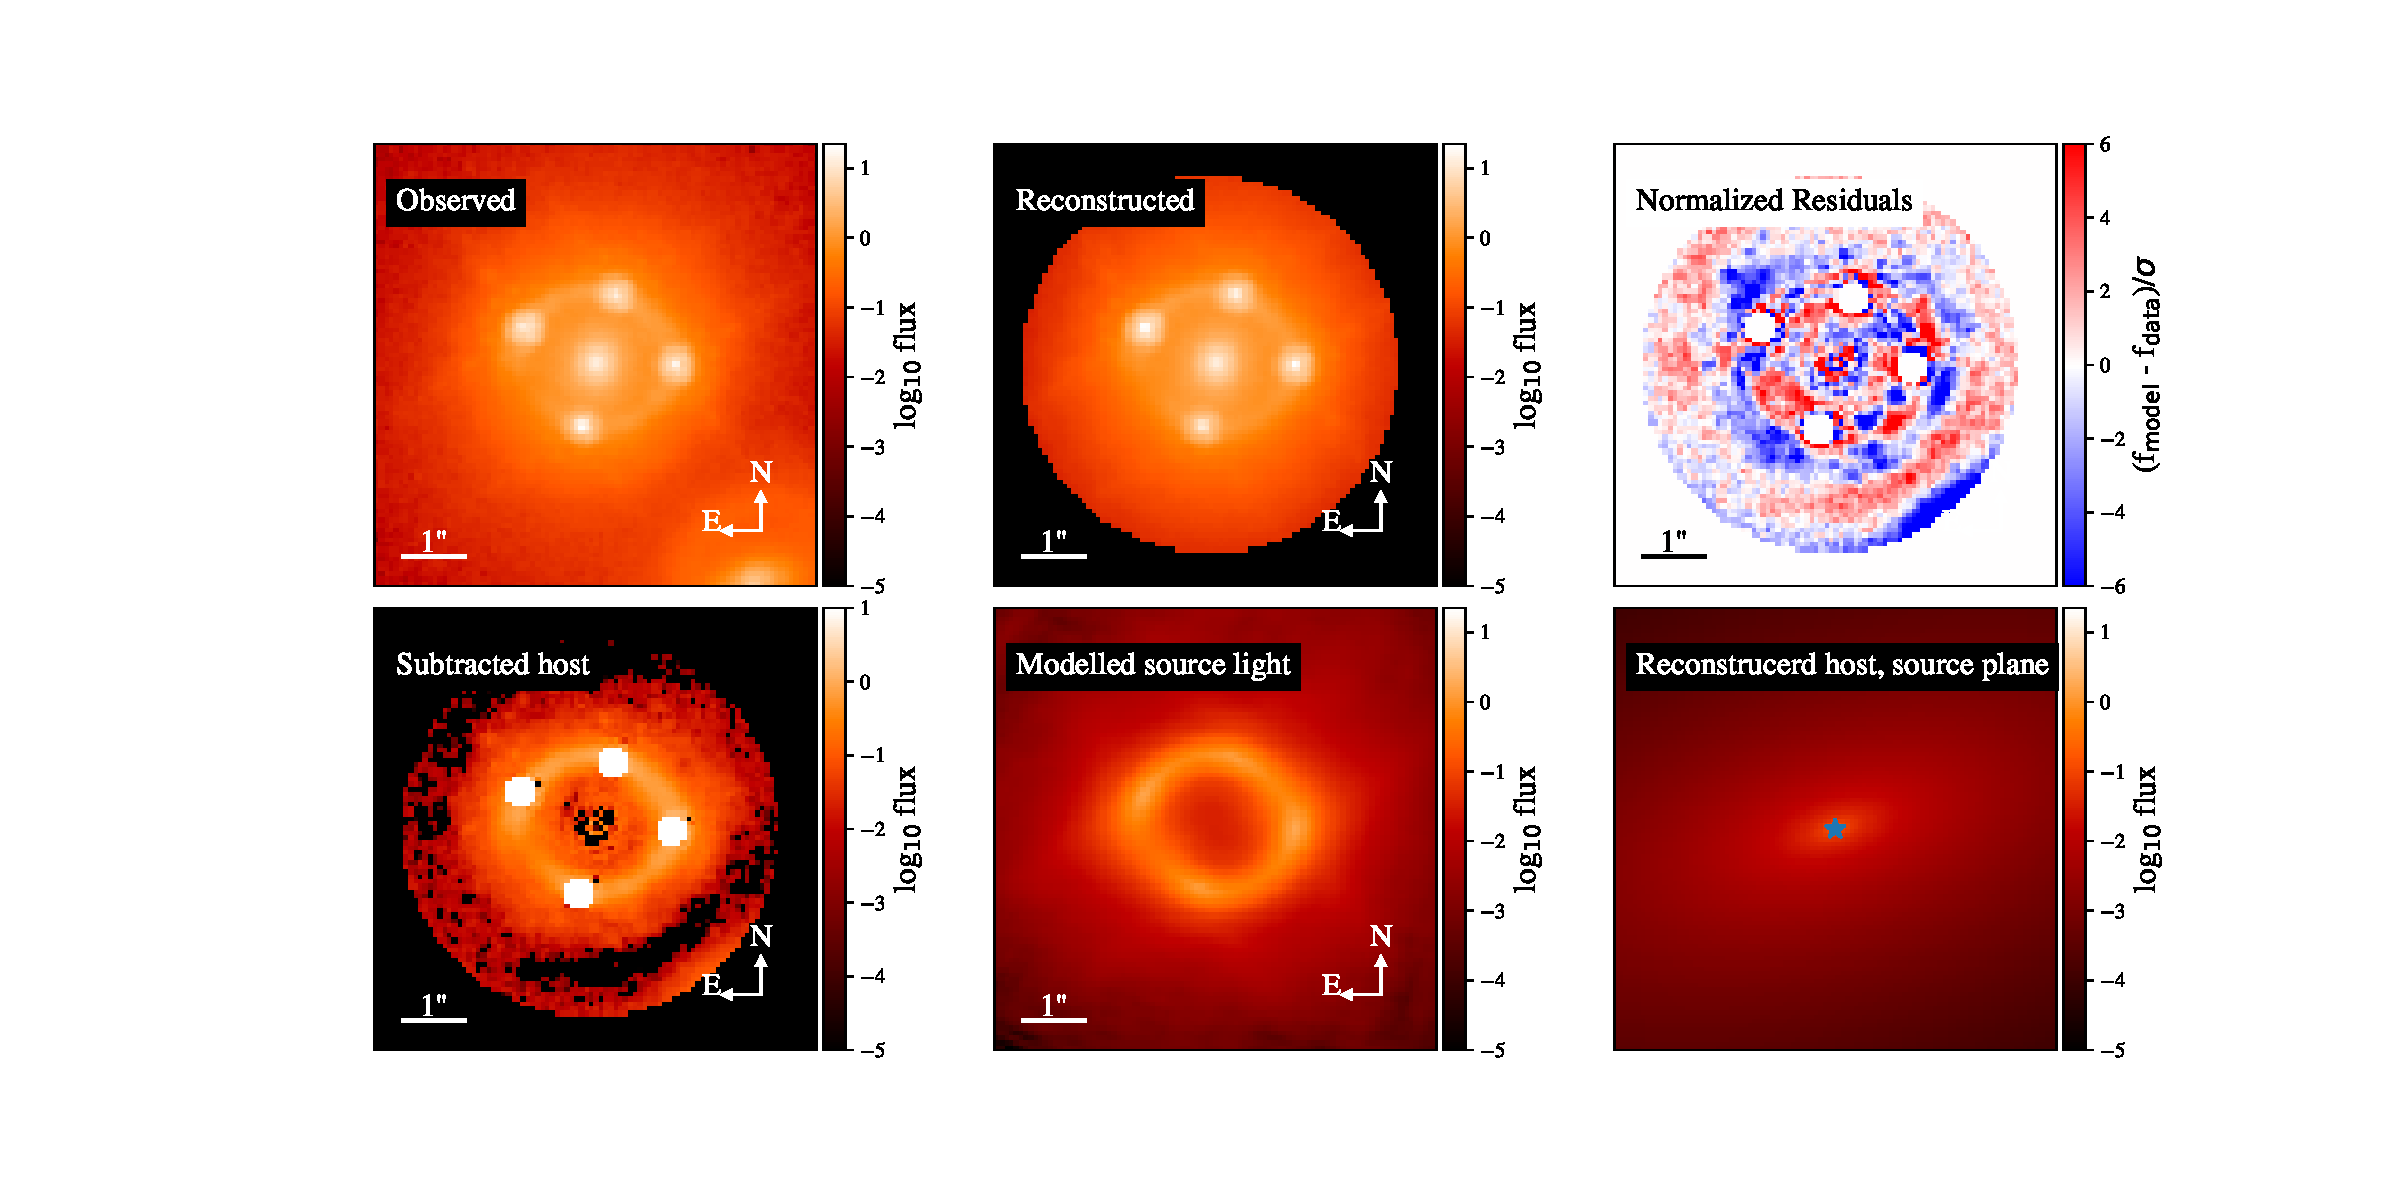
\includegraphics[trim = 40mm 25mm 40mm 25mm, clip, width=0.5\textwidth]{fig/HE0435_best_inference.pdf}}&
\subfloat[RXJ1131]{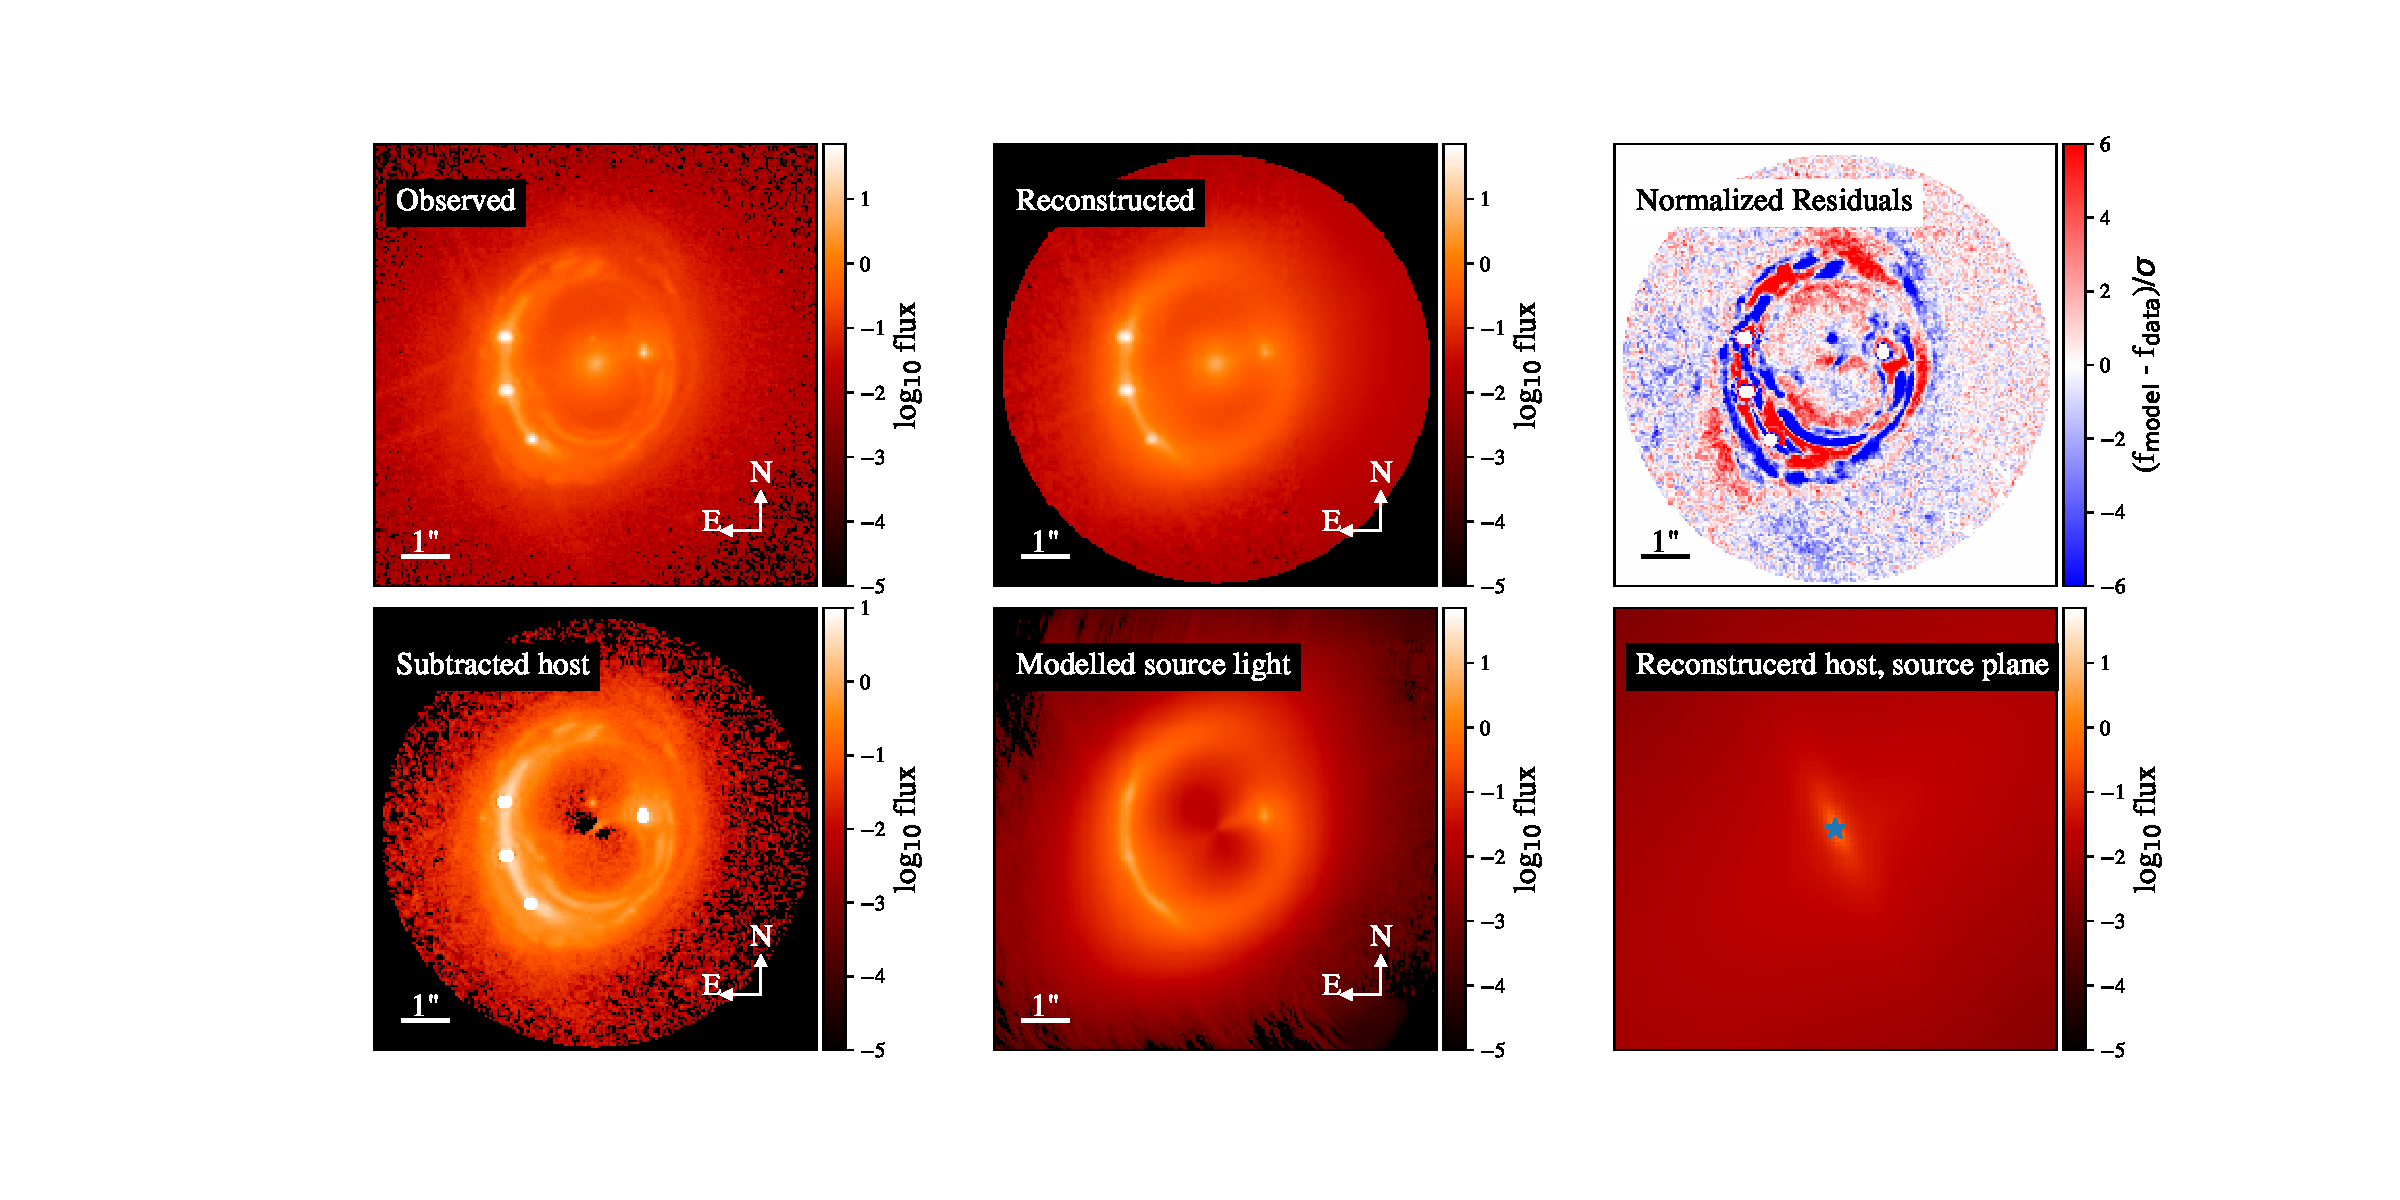
\includegraphics[trim = 40mm 25mm 40mm 25mm, clip, width=0.5\textwidth]{fig/RXJ1131_best_inference.pdf}}\\
\subfloat[WFI2033]{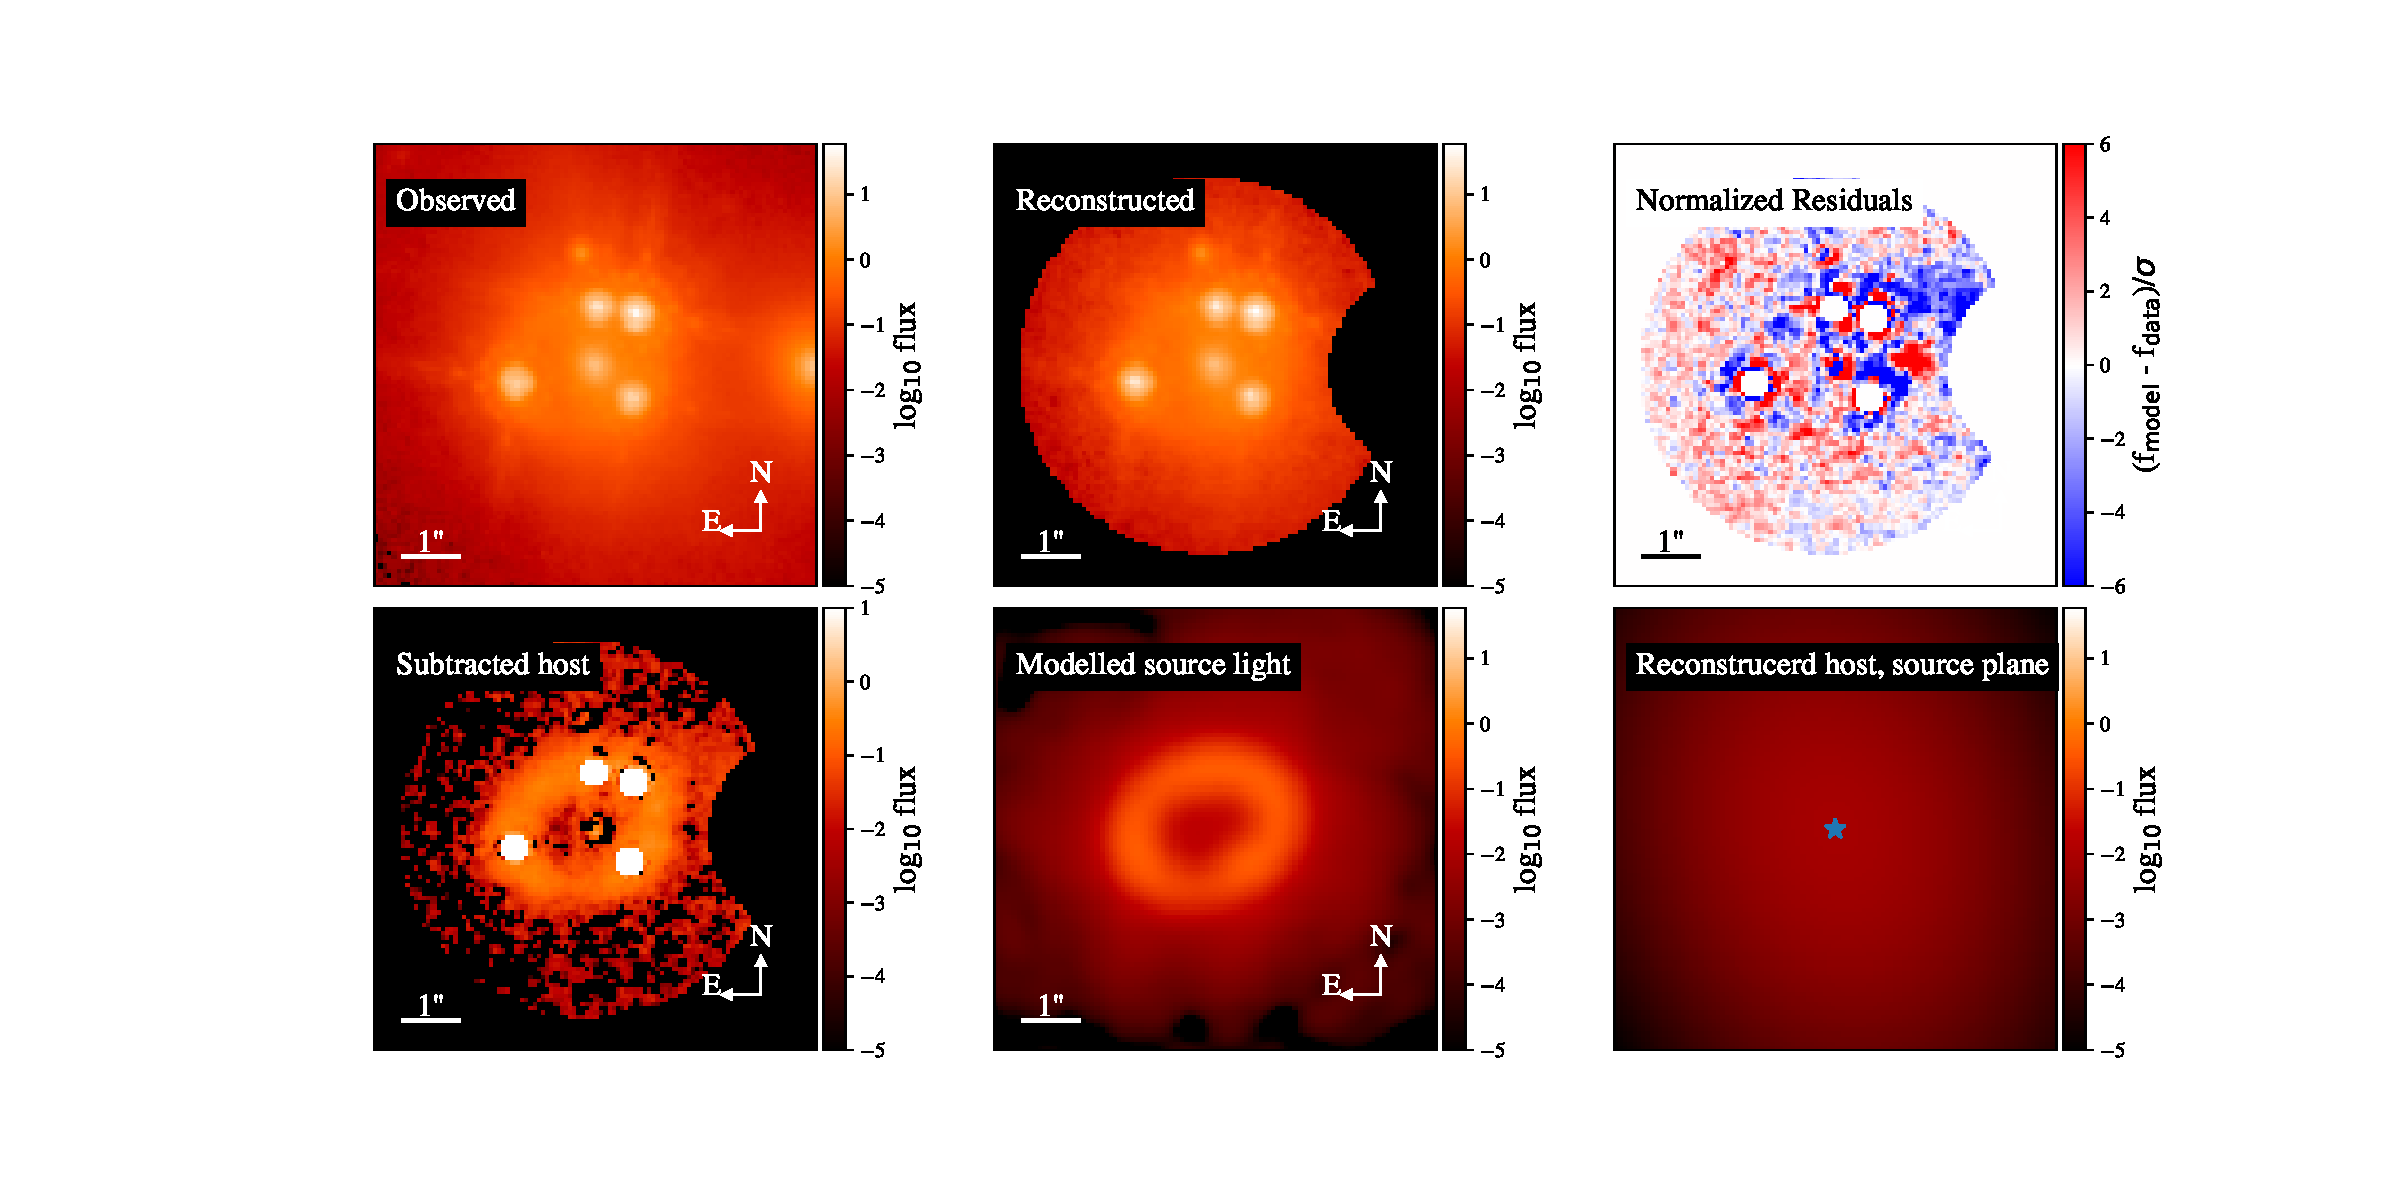
\includegraphics[trim = 40mm 25mm 40mm 25mm, clip, width=0.5\textwidth]{fig/WFI2033_best_inference.pdf}}&
\subfloat[SDSS1206]{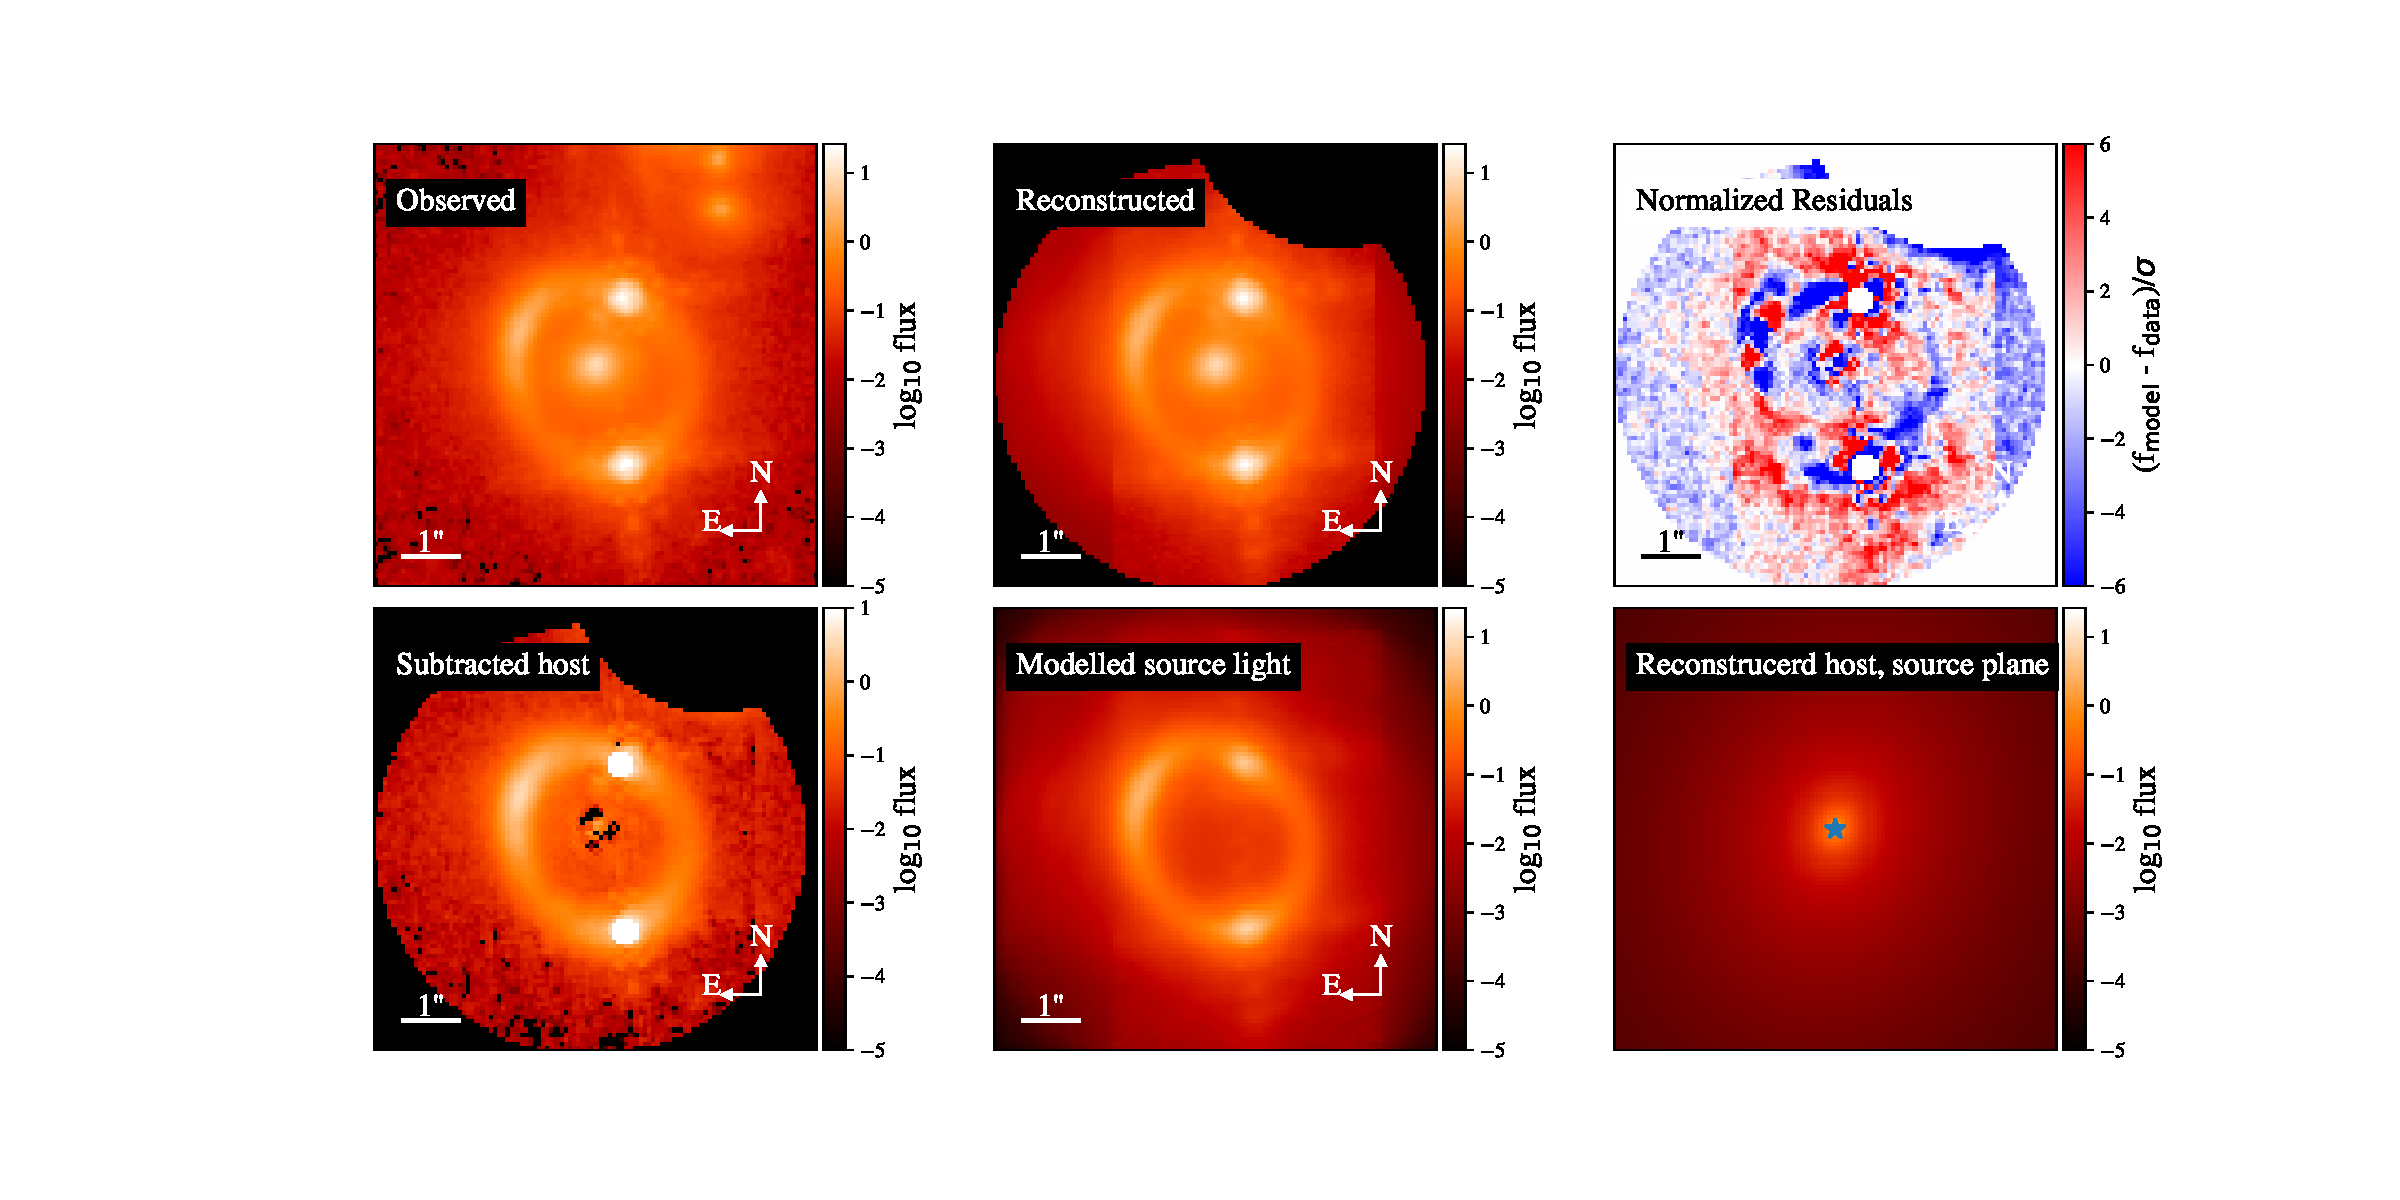
\includegraphics[trim = 40mm 25mm 40mm 25mm, clip, width=0.5\textwidth]{fig/SDSS1206_best_inference.pdf}}\\
\subfloat[HE1104]{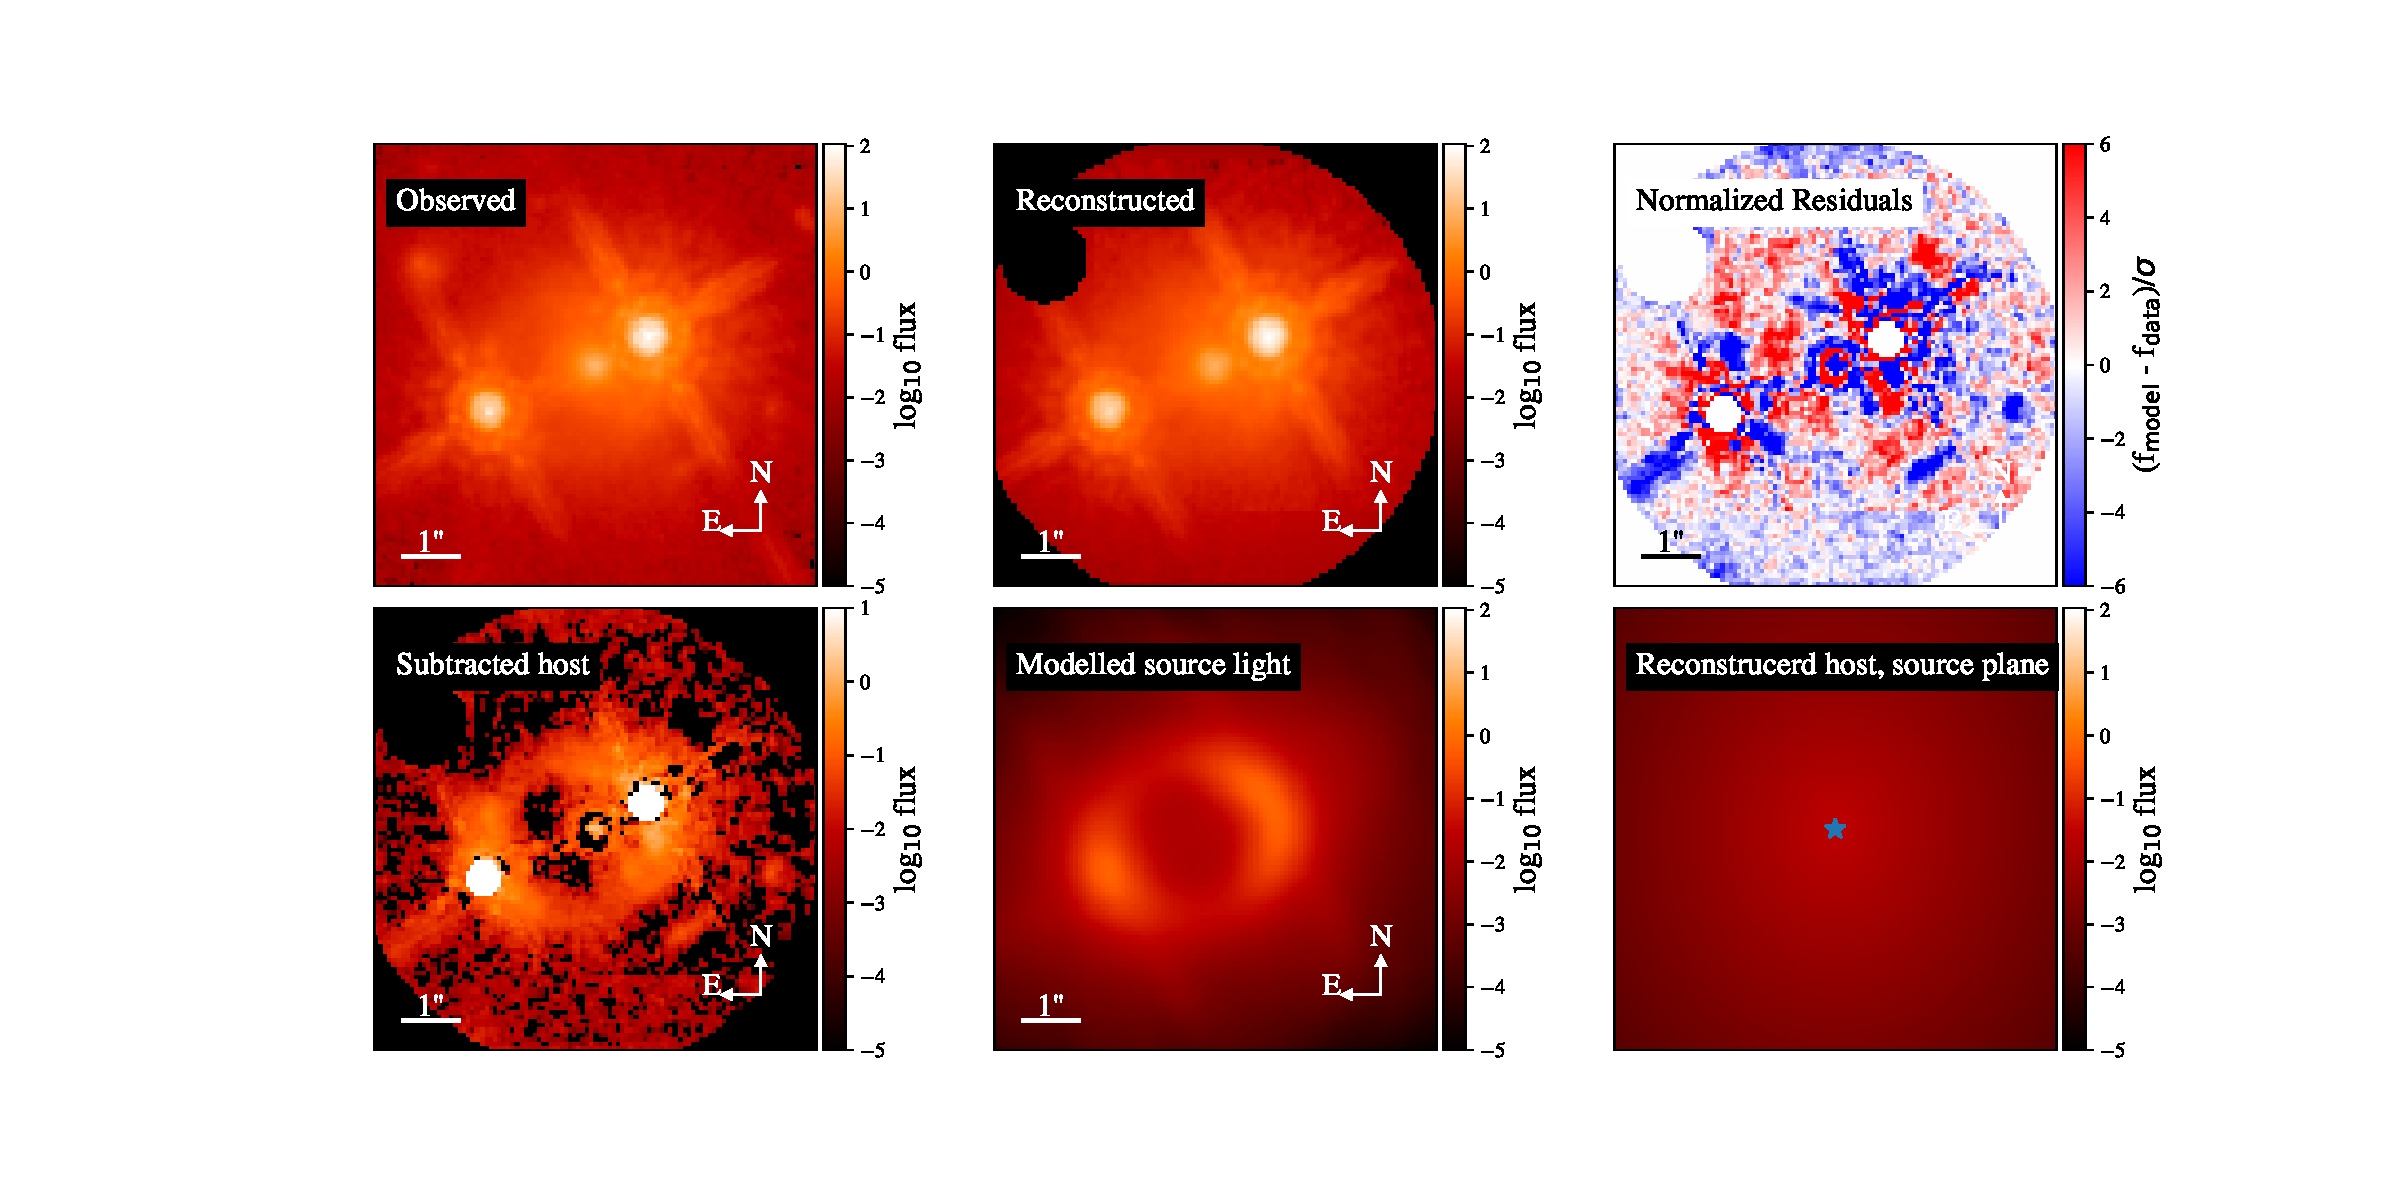
\includegraphics[trim = 40mm 25mm 40mm 25mm, clip, width=0.5\textwidth]{fig/HE1104_best_inference.pdf}}&
\subfloat[SDSS0246]{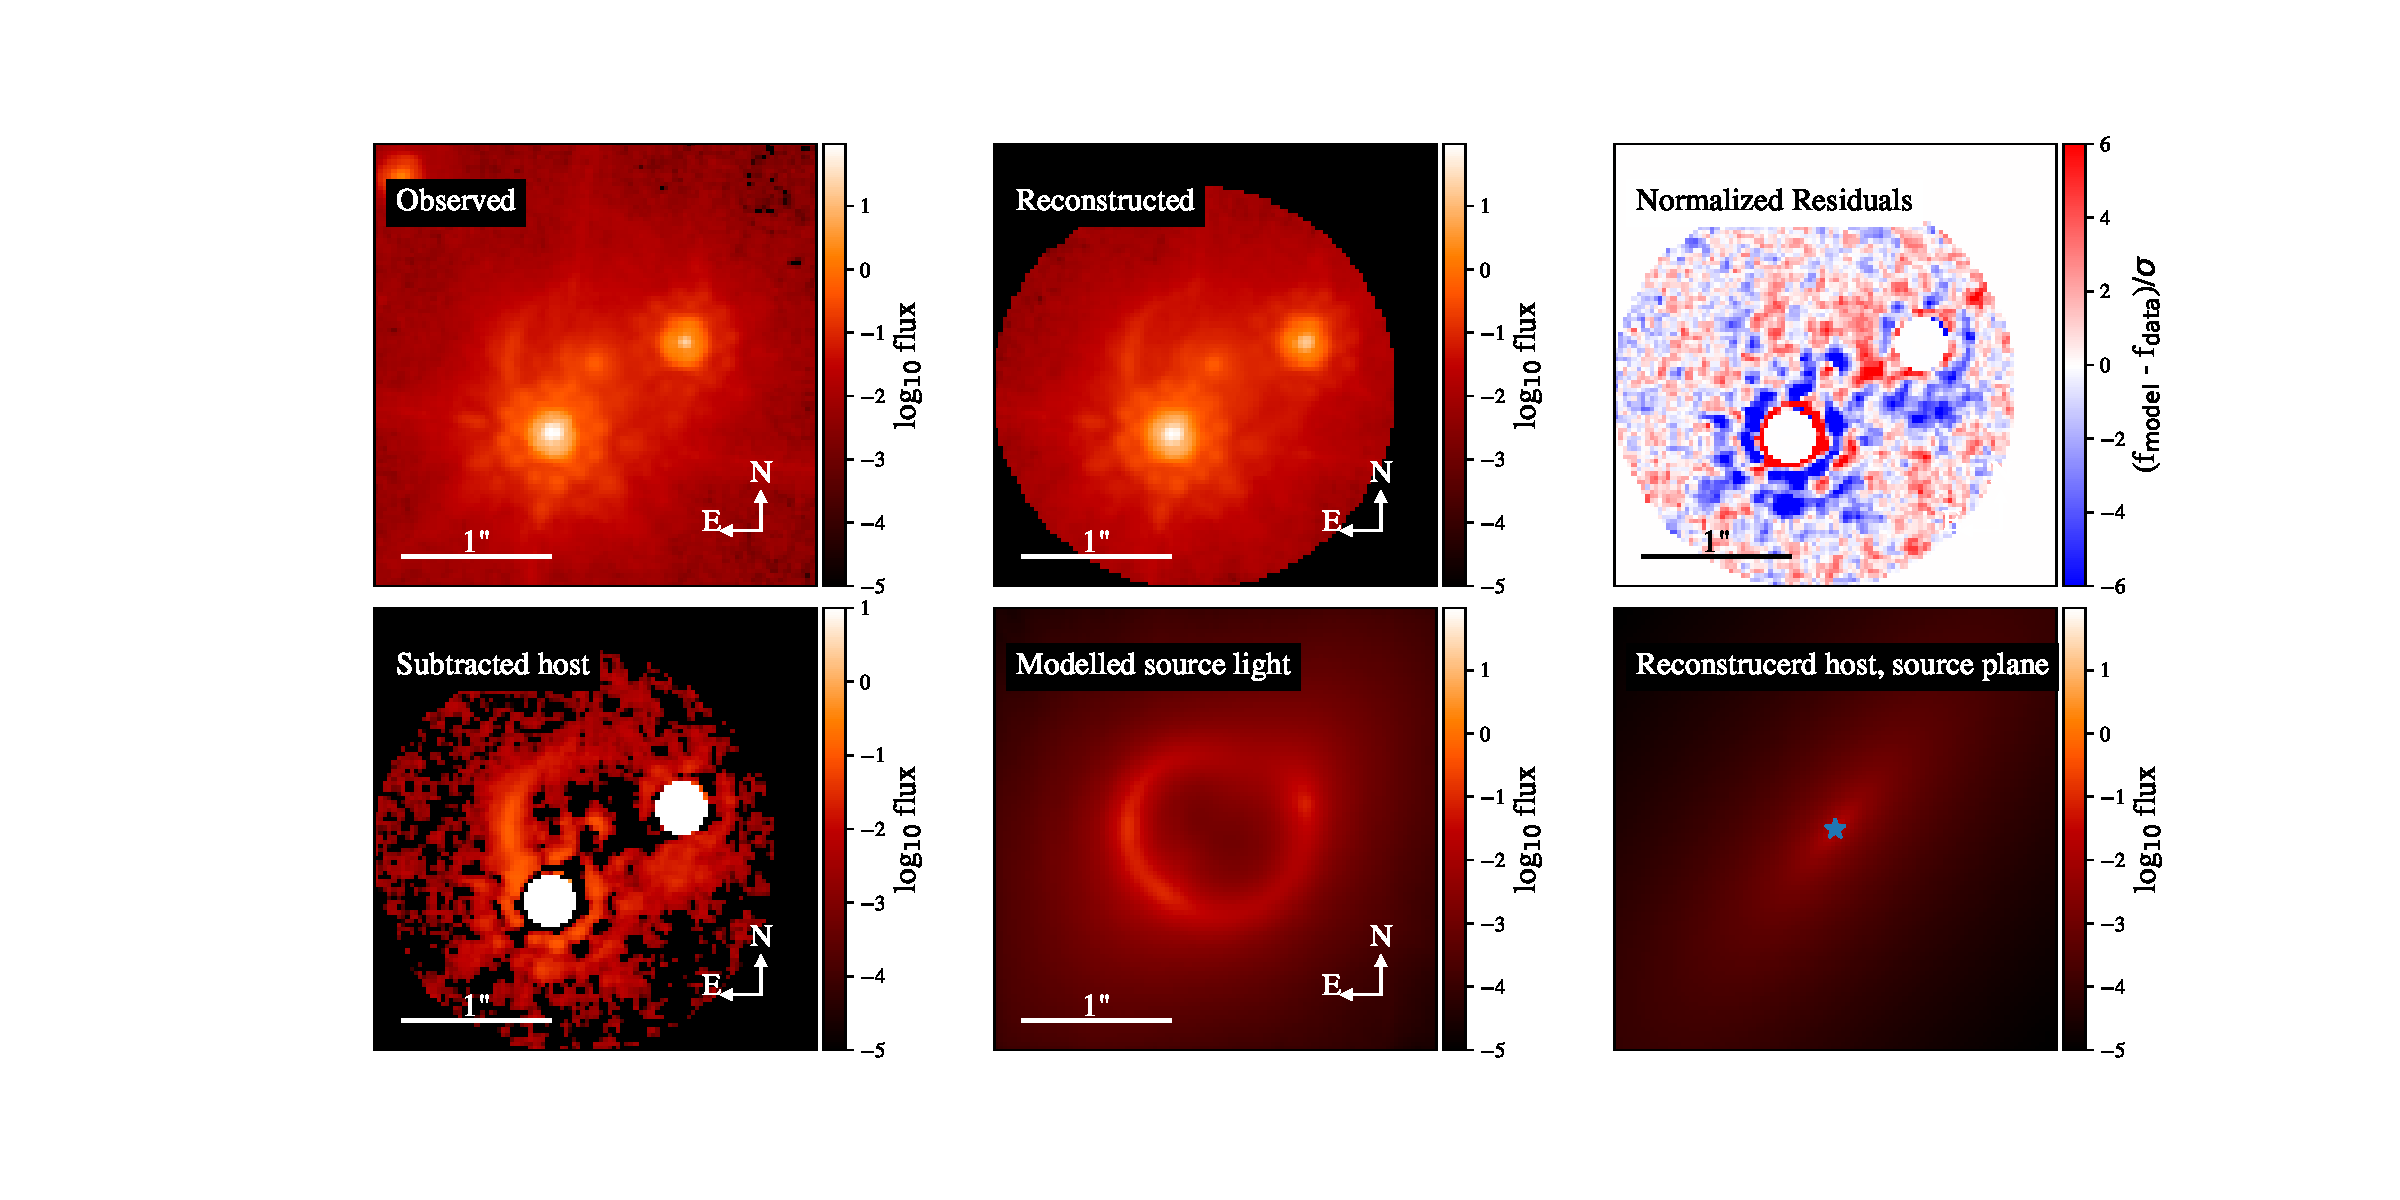
\includegraphics[trim = 40mm 25mm 40mm 25mm, clip, width=0.5\textwidth]{fig/SDSS0246_best_inference.pdf}}\\
\subfloat[HS2209]{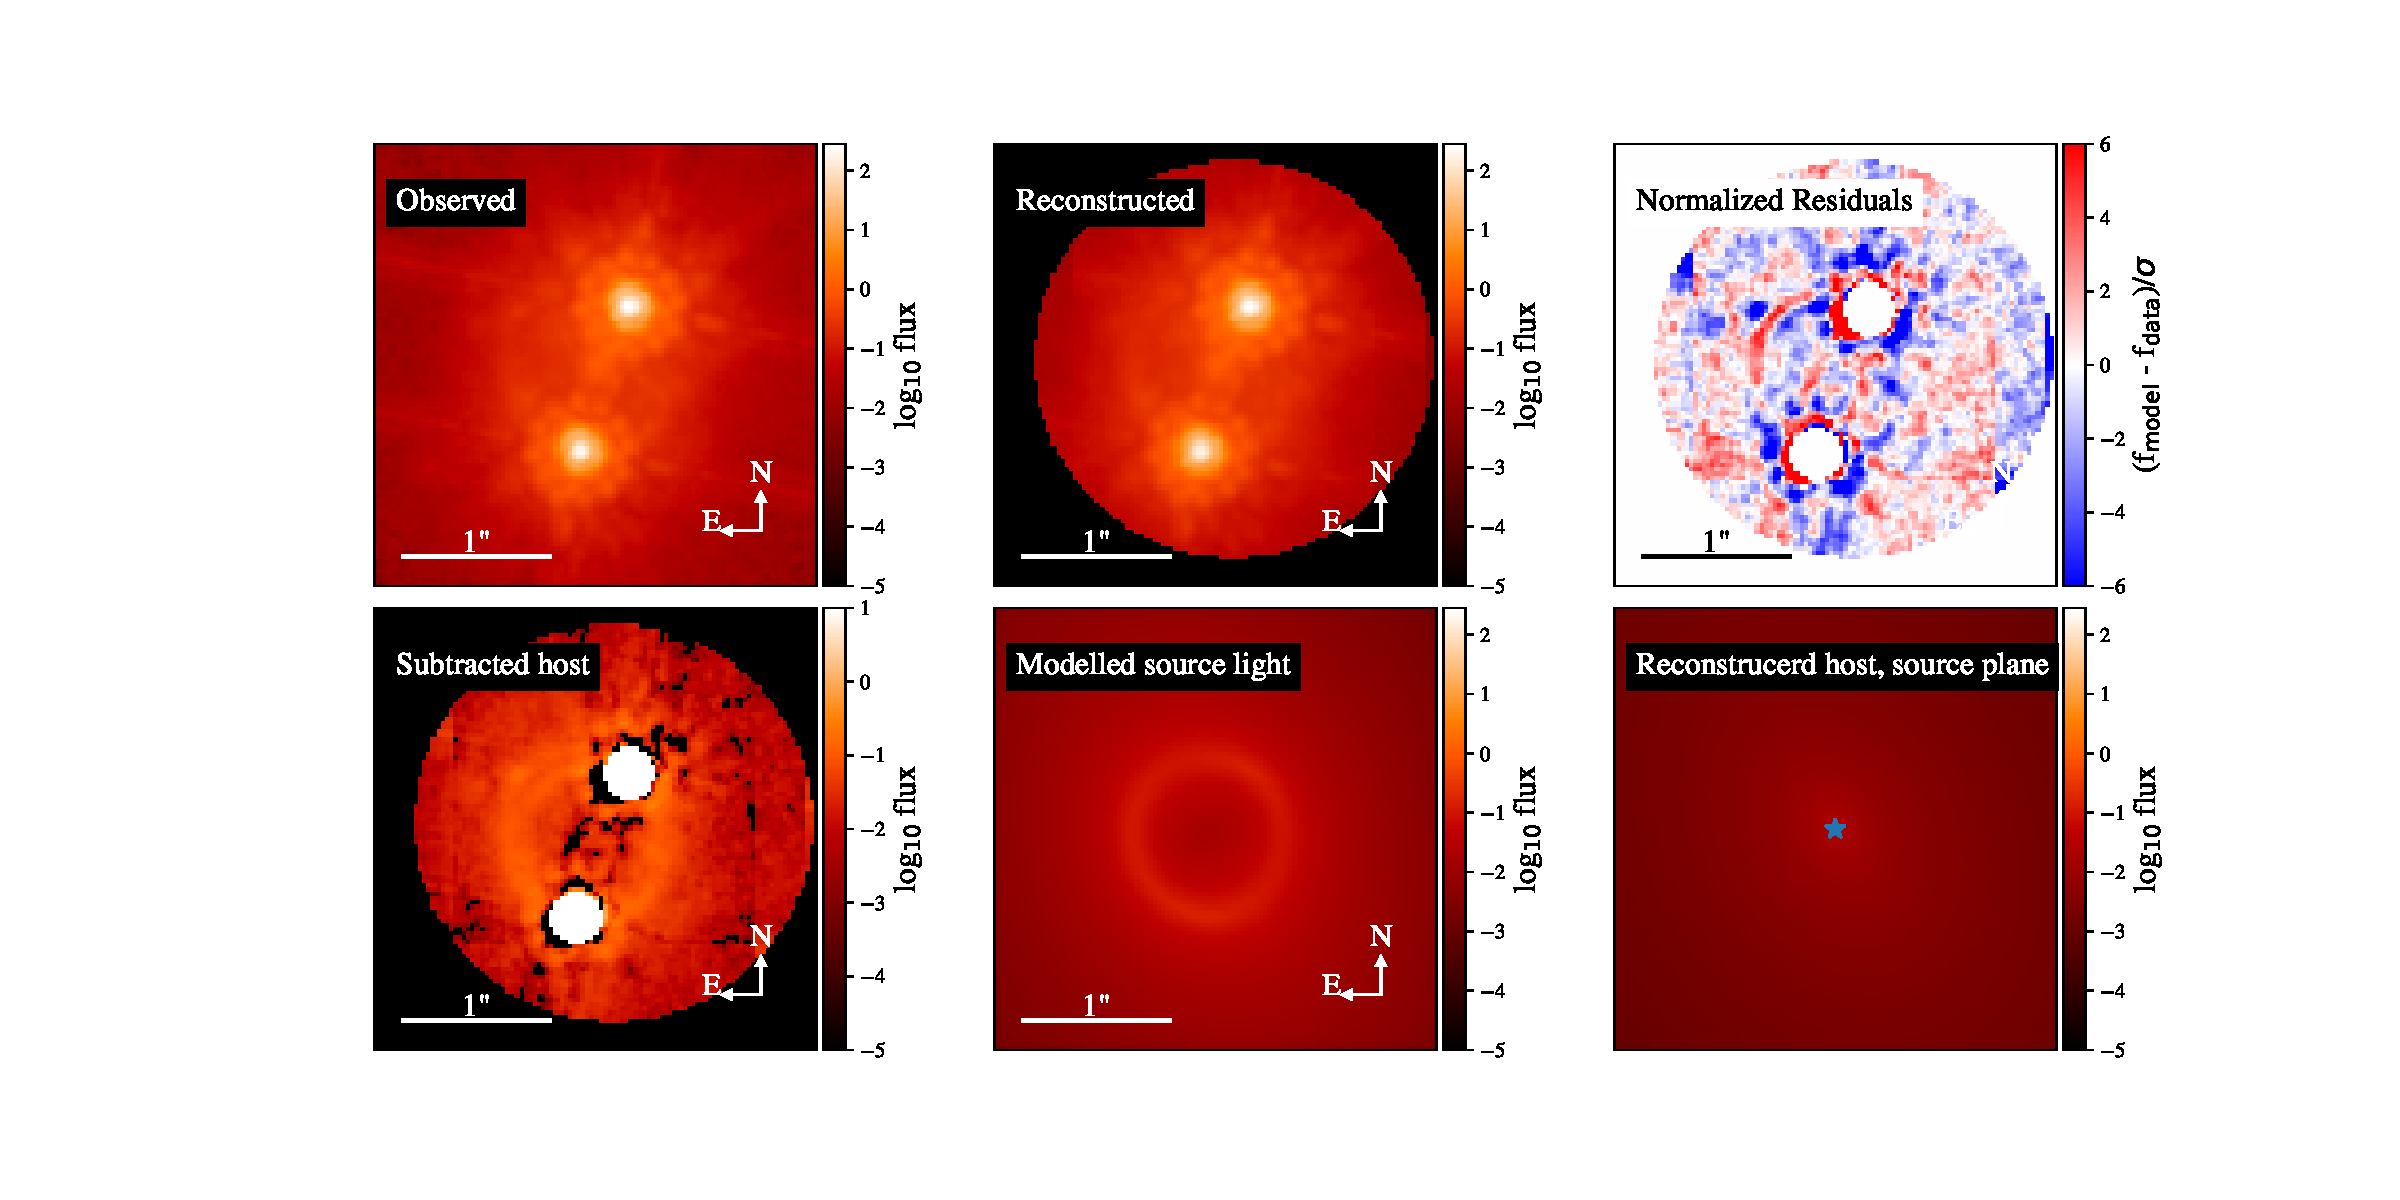
\includegraphics[trim = 40mm 25mm 40mm 25mm, clip, width=0.5\textwidth]{fig/HS2209_best_inference.pdf}}&
\subfloat[HE0047]{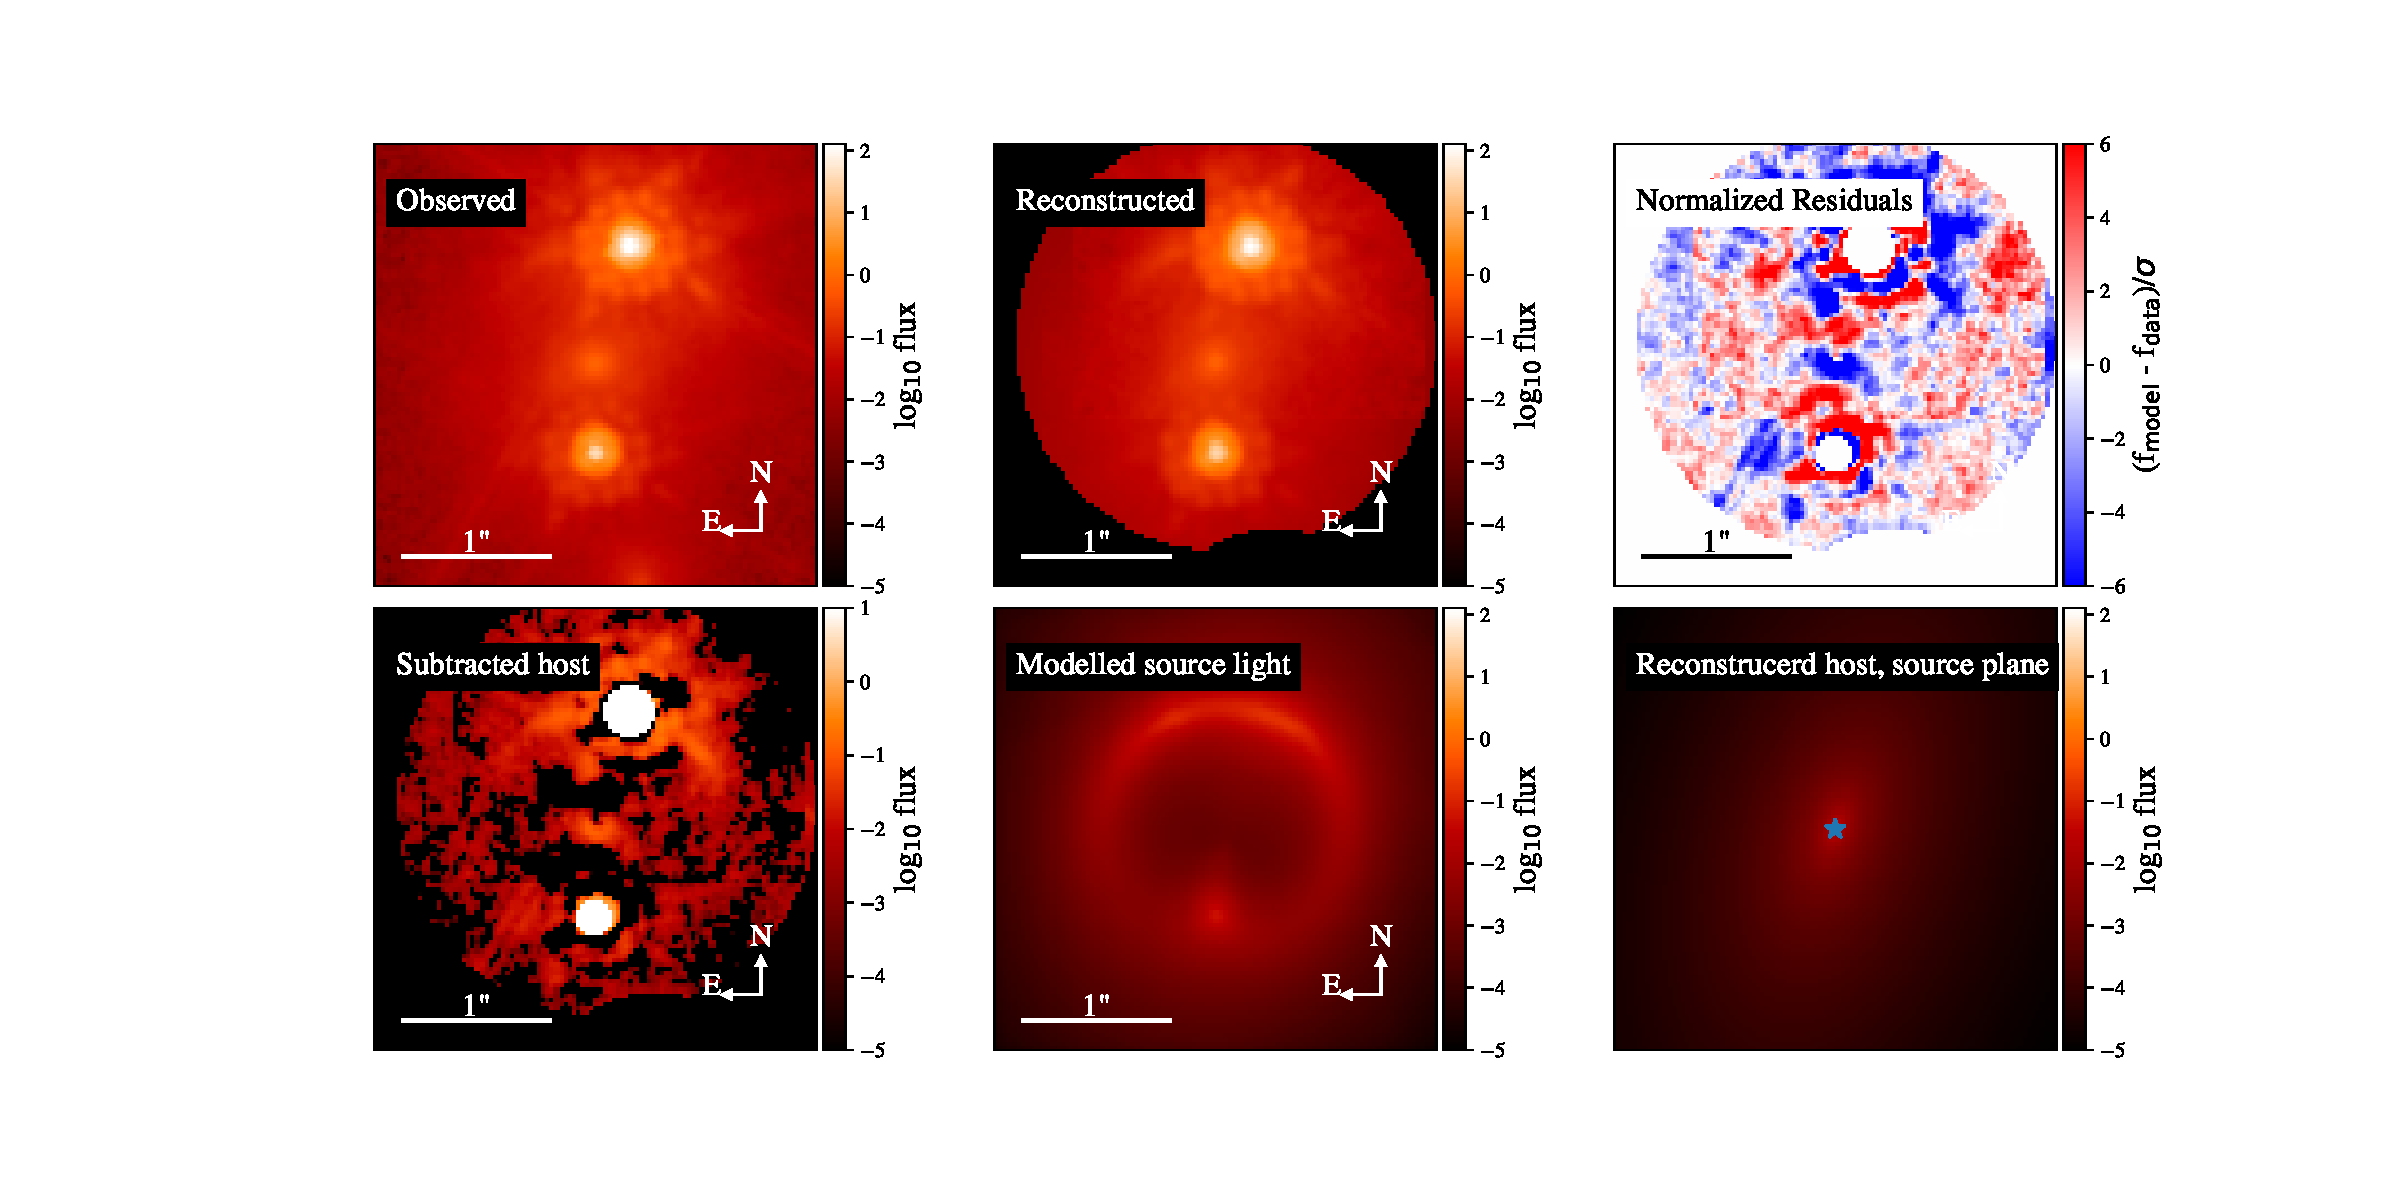
\includegraphics[trim = 40mm 25mm 40mm 25mm, clip, width=0.5\textwidth]{fig/HE0047_best_inference.pdf}}\\
\end{tabular}
\caption{\label{fig:image_inference} 
Something}
\end{figure*} 

\subsubsection{RXJ1131}


\subsubsection{WFI2033}
The objects which is close to the lens, we model its light as one extended source described by \sersic\ profile. 


\subsubsection{SDSS1206}

\subsubsection{HE1104}

\subsubsection{SDSS0246}

\subsubsection{HE0047}

\subsubsection{HS2209}

The comparison to the previous fitting.

We summarized the inference for the eight systems in the table.
name--Setts--BestFitChisq--Totalflux-- Host ratio --Reff--Sersicn--magnitude - Stellar mass

\begin{table*}
\renewcommand{\arraystretch}{1.5}
%\setlength{\tabcolsep}{20pt}
\centering
  \begin{threeparttable}
\caption{Summary of lensed AGN inference.}\label{data_set}    
%\resizebox{12cm}{!}{
     \begin{tabular}{ccccccc}
\hline
Object ID & Magnitude & Host-Total Flux Ratio & Reff & \sersic\ $n$ & adopted AGE & $\log (M_{*}$)  \\
 & (AB system) & ($\%$) & (arcsec) & & (Gyr) & (M$_{\odot}$) \\ \hline
HE0435 & $21.332\substack{+0.208\\-0.175}$ & $62.471\pm10.893$ & $0.298\pm0.027$ & $2.829\pm0.251$ & $1.500$ & $10.98\substack{+0.07\\-0.08}$ \\
RXJ1131$_{\rm bulge}$ & $22.074\substack{+0.164\\-0.142}$ & $6.634\pm0.929$ & $0.106\pm0.007$ & fix to 4 & $3.000$ & $1.01\substack{+0.06\\-0.07}$ \\
RXJ1131$_{\rm disk}$ & $19.305\substack{+0.154\\-0.135}$ & $84.939\pm11.241$ & $0.875\pm0.062$ & fix to 1 & $1.500$ & $1.04\substack{+0.05\\-0.06}$ \\
WFI2033 & $21.404\substack{+0.167\\-0.145}$ & $35.723\pm5.093$ & $0.294\pm0.025$ & $0.528\pm0.011$ & $0.625$ & $10.66\substack{+0.06\\-0.07}$ \\
SDSS1206 & $21.287\substack{+0.222\\-0.184}$ & $32.286\pm5.977$ & $0.110\pm0.020$ & $4.526\pm0.555$ & $0.625$ & $10.78\substack{+0.07\\-0.09}$ \\
HE1104 & $21.274\substack{+0.188\\-0.160}$ & $14.142\pm2.250$ & $0.265\pm0.026$ & $1.033\pm0.034$ & $0.625$ & $11.04\substack{+0.06\\-0.08}$ \\
SDSS0246 & $23.575\substack{+0.394\\-0.289}$ & $3.756\pm1.143$ & $0.381\pm0.098$ & $4.963\pm0.048$ & $0.626$ & $10.69\substack{+0.12\\-0.16}$ \\
HS2209 & $20.385\substack{+0.262\\-0.211}$ & $19.454\pm4.165$ & $1.921\pm1.070$ & $2.953\pm0.438$ & $1.001$ & $11.18\substack{+0.08\\-0.10}$ \\
HE0047 & $22.972\substack{+0.626\\-0.394}$ & $2.496\pm1.093$ & $0.282\pm0.176$ & $3.603\pm1.533$ & $0.625$ & $10.89\substack{+0.16\\-0.25}$ \\
\hline
\end{tabular}
%}
\begin{tablenotes}
      \small
      \item Note: $-$ If any
\end{tablenotes}    
\end{threeparttable}
\end{table*}




\subsection{Stellar mass estimates}
For those ones have multi-bands, we attempt to infer the color of the host in the image plane.

How do we infer the color? All the available bands? Which is dominating the scatter?

\section{Black Hole mass estimates}
We use viral method to estimate the mass of the black hole. The board-line adopted. We aim to adopt the self-consistent to recalibrate the \mbh~of our sample. 
[] The recipes. [] The board lines and the resulting BH mass and listed in the table. []The summarizing table.

\section{Results}
%estimate the black hole mass.

%scaling relation and compare to the Ding+20

%\ding{Do we consider the Selection effect? We only select 8 sample? Maybe we only over plot them together and see if the results are self-consistent?}

\section{Discussion and Conclusion}
[] This work confirm the bright future of lensing.



\section*{Acknowledgements}

The Acknowledgements section is not numbered. Here you can thank helpful
colleagues, acknowledge funding agencies, telescopes and facilities used etc.
Try to keep it short.

%%%%%%%%%%%%%%%%%%%%%%%%%%%%%%%%%%%%%%%%%%%%%%%%%%

%%%%%%%%%%%%%%%%%%%% REFERENCES %%%%%%%%%%%%%%%%%%

% The best way to enter references is to use BibTeX:

\bibliographystyle{mnras}
\bibliography{reference} % if your bibtex file is called example.bib


% Alternatively you could enter them by hand, like this:
% This method is tedious and prone to error if you have lots of references
%\begin{thebibliography}{99}
%\bibitem[\protect\citeauthoryear{Author}{2012}]{Author2012}
%Author A.~N., 2013, Journal of Improbable Astronomy, 1, 1
%\bibitem[\protect\citeauthoryear{Others}{2013}]{Others2013}
%Others S., 2012, Journal of Interesting Stuff, 17, 198
%\end{thebibliography}

%%%%%%%%%%%%%%%%%%%%%%%%%%%%%%%%%%%%%%%%%%%%%%%%%%

%%%%%%%%%%%%%%%%% APPENDICES %%%%%%%%%%%%%%%%%%%%%

\appendix

\section{Color inference of the host}
We took the other band data and get the only arc image. We adopt these image and do the SED fitting to get the color information.

%%%%%%%%%%%%%%%%%%%%%%%%%%%%%%%%%%%%%%%%%%%%%%%%%%


% Don't change these lines
\bsp	% typesetting comment
\label{lastpage}
\end{document}

% End of mnras_template.tex